\FloatBarrier
\subsection{Native implementation, complete checking and Python integration}\label{sec:native-evidence}
% Internal experiment: /home/onyr/code/phd/numerical-checker-contracts-investigation/native/s124/{dyadic.hpp,bindings.cpp,CMakeLists.txt,build.py,reference.py} and scripts/s124_native_{runtime,conformance,validate,report}.py. Results: newresults/s124-native/. The original Python census in newresults/s124-cost-runtime/ is preserved unchanged.
We extend the objective experiment with a native implementation and complete retained-solution checking on the same 296 instances. We retain all earlier Python objective measurements, tables and figures. This pilot uses C++20 with GCC/G++ 15.2.0, Boost 1.89.0 and pybind11 3.1.0 on the same x86-64 host with Python 3.13.13. We follow the existing Kayros/PyVRP pattern of an owned native data model behind pybind11 bindings, without changing either solver or the production MAMUT library.

\subsubsection{Exact arithmetic, range bounds and boundary behavior}
We decode each finite nonnegative binary64 quantity into an integer significand and a binary exponent, including subnormals and signed zero. We select a common scale $2^q$ over every arc cost, time-window bound and service duration. This produces exact integer operands without floating-point multiplication or rounding. Let $A$, $E$, $L$ and $S$ denote the maximum scaled arc cost, earliest time, latest time and service duration. For an instance with $n$ customers, we use the conservative bound
\[
    B = \max\!\left\{2nA,\ E+(n+1)(A+S)\right\}.
\]
Every structurally valid solution has at most $n$ nonempty routes and hence at most $2n$ arcs in total. A route has at most $n+1$ arcs and $n$ customer service contributions. The historical pilot allowed an additional service term in its conservative bound. Under this specification that depot term is zero. Expanding the waiting recurrence bounds every arrival or departure by the largest earliest time plus the accumulated arc and service contributions. Hence $B$ bounds the objective and temporal intermediates for this instance, rather than only the retained incumbent. We also require $L$ to fit the chosen representation.

When $\max\{B,L\}\leq 2^{127}-1$, the prototype uses Boost's fixed-width unsigned 128-bit storage with a reserved sign bit and explicit checked additions. Otherwise, it prepares arbitrary-precision integer operands. A checked-add overflow also triggers an arbitrary-precision retry before a result is accepted. Capacity checks compare each demand with remaining capacity before addition. The pilot supports resource integers that are exactly representable in binary64 and lie between 0 and the signed 64-bit maximum, and caps the customer count at $10^6$ subject to available memory. It rejects unsupported resource widths explicitly. This supported domain is a restriction of the general reference, rather than a claim to implement every static input accepted by the specification.

The boundary suite checks every finite binary64 exponent class, subnormal bit positions, mixed-exponent sums, signed zero, nonfinite rejection, exact objectives beyond finite binary64, and checked-overflow fallback. It compares feasibility and exact costs with the frozen Python reference on depot/service, time-window, capacity, fleet and structural witnesses. In particular, the rounded checker accepts a constructed deadline case that the exact checker rejects. We also check native ownership of matrix and route data, so later mutations of the supplied Python objects cannot silently change the prepared model. The independent suite contains 2496 passing checks, and 67 standalone core checks pass under address and undefined-behavior sanitizers with standard-library assertions. These tests are evidence for the recorded build, rather than certification of every compiler or platform.

\subsubsection{Measurement scopes and integration boundaries}
We run 2 sequential fresh processes over all 296 instances, with 5 warm-ups and 9 randomized measured blocks per cell, a 20 ms calibration target and seed 2026102607. The native extension uses optimized C++20 without fast-math or floating-point contraction, and without a host-specific architecture flag. We measure 6 native operations: flat binary64 objective evaluation, exact objective evaluation with per-arc conversion or a prepared integer matrix, and complete solution checking with each of those 3 arithmetic paths. The rounded full checker is a separately identified numerical diagnostic.

The complete checker validates nonempty routes, exact customer coverage, duplicates, fleet size, capacity, depot initialization, service durations, all customer and return time windows, and the objective. Input parsing, instance validation, matrix packing and numeric preparation remain outside the solution-checking timers. Table~\ref{tab:native-preparation} reports those preparation costs separately. The native model owns both a binary64 matrix and its exact integer materialization. The full Python reference additionally parses the original JSON tokens and constructs a Fraction matrix, so its preparation column includes different work.

For each native operation, we measure a C++ batch and repeated Python calls through pybind11. The C++ timer runs inside the batch, excluding its single Python binding call and result wrapping. A compiler signal fence and an independently checked result checksum prevent the benchmark from discarding the repeated evaluations. Scalar binding calls include per-call dispatch and native-result wrapping. They retain the Global Interpreter Lock (GIL), while a batch releases it once around the repeated native work. Separate measurements add conversion of Python route lists on every complete check, then extraction and normalization of the exact Python hierarchical ranking key. The frozen Python reference also performs its existing canonical sorting and returned-route copies. These are measured implementation boundaries, rather than identical serialization pipelines.

\begin{figure}[htbp]
\centering
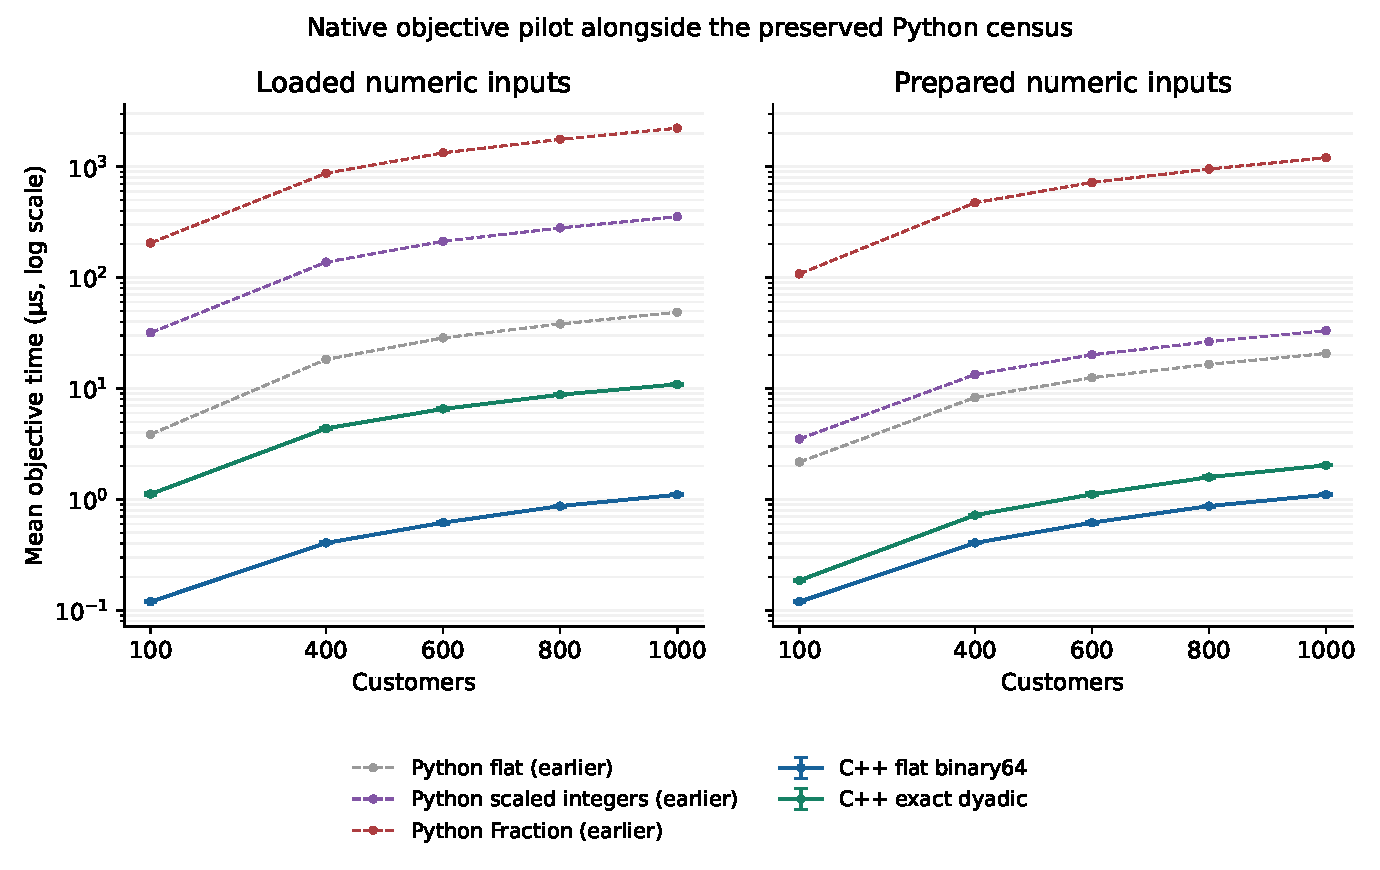
\includegraphics[width=\linewidth]{figures/native-objective-by-size.pdf}
\caption{Native objective evaluation alongside the preserved Python census, with logarithmic time axes. Native error bars span the 2 process means. The native prepared scope traverses a full integer matrix, while the earlier Python prepared scope reduces gathered route operands. Dashed Python curves retain the earlier processes and provide implementation context rather than simultaneous paired comparisons.}\label{fig:native-objectives}
\end{figure}

\begin{figure}[htbp]
\centering
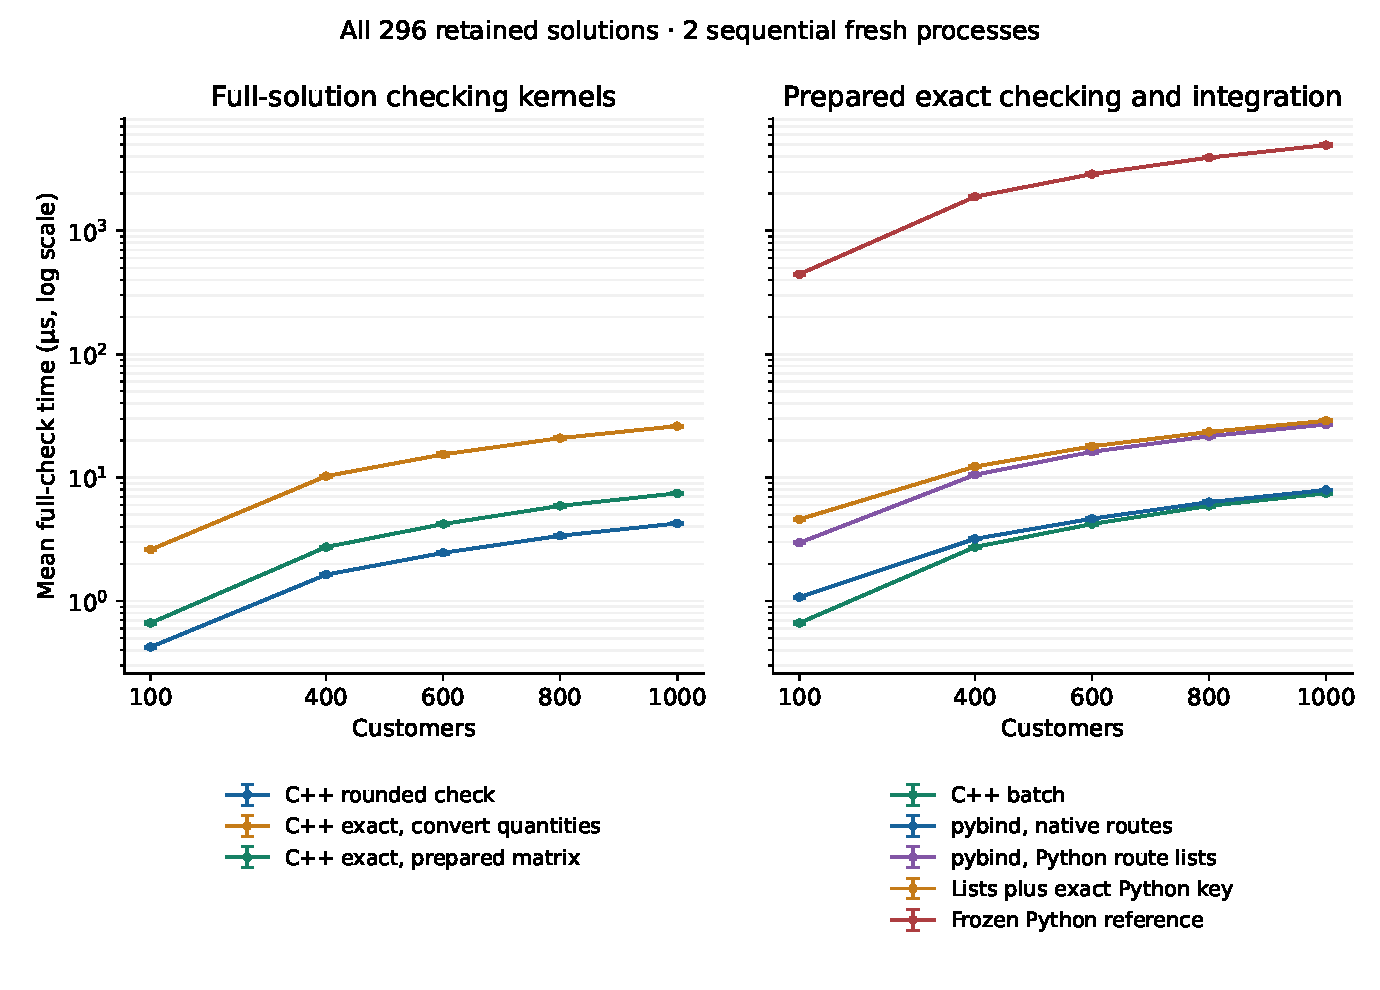
\includegraphics[width=\linewidth]{figures/native-checking-by-size.pdf}
\caption{Complete checking and Python integration on every retained solution at each requested size. The left panel compares concrete native arithmetic paths. The right panel separates native batches, scalar bindings, route-list conversion, exact-key extraction and the frozen Python reference. Error bars span process means and are not confidence intervals.}\label{fig:native-checking}
\end{figure}

\begin{table}[htbp]
\centering\small
\begin{tabularx}{\linewidth}{@{}Xrrrrr@{}}
\toprule
Implementation & 100 & 400 & 600 & 800 & 1000\\
\midrule
Flat binary64 objective & 0.120 & 0.405 & 0.618 & 0.871 & 1.102\\
Exact objective, convert arcs & 1.117 & 4.363 & 6.540 & 8.786 & 10.896\\
Exact objective, prepared matrix & 0.186 & 0.722 & 1.111 & 1.588 & 2.031\\
Rounded full check & 0.424 & 1.636 & 2.459 & 3.380 & 4.253\\
Exact full check, convert quantities & 2.606 & 10.277 & 15.412 & 20.899 & 26.139\\
Exact full check, prepared matrix & 0.664 & 2.739 & 4.209 & 5.902 & 7.467\\
\bottomrule
\end{tabularx}
\caption{Pure C++ batches: mean time in $\mu$s per complete solution, by customer count. The timer excludes the single batch binding call and result wrapping. Rounded checks are diagnostics with different numerical semantics.}\label{tab:native-kernels}
\end{table}

\begin{table}[htbp]
\centering\small
\begin{tabularx}{\linewidth}{@{}Xrrrrr@{}}
\toprule
Implementation & 100 & 400 & 600 & 800 & 1000\\
\midrule
Flat binary64 objective & 0.517 & 0.851 & 1.095 & 1.353 & 1.593\\
Exact objective, convert arcs & 1.530 & 4.797 & 7.005 & 9.208 & 11.348\\
Exact objective, prepared matrix & 0.584 & 1.135 & 1.534 & 2.024 & 2.462\\
Rounded full check & 0.827 & 2.054 & 2.918 & 3.856 & 4.722\\
Exact full check, convert quantities & 3.021 & 10.780 & 15.948 & 21.398 & 26.661\\
Exact full check, prepared matrix & 1.076 & 3.189 & 4.647 & 6.329 & 7.938\\
Prepared exact check, Python route lists & 2.966 & 10.539 & 16.202 & 21.649 & 26.951\\
Route lists and exact Python ranking key & 4.597 & 12.288 & 17.928 & 23.438 & 28.891\\
Frozen Python reference full check & 444.597 & 1884.382 & 2875.155 & 3912.013 & 4939.869\\
\bottomrule
\end{tabularx}
\caption{Python integration: mean time in $\mu$s per complete solution. The first 6 rows call the same native kernels through pybind11 on prepared native route objects. The final rows add route-list conversion, exact-key extraction, or use the frozen Fraction reference, whose sorting and output copies are included.}\label{tab:native-integration}
\end{table}

\begin{table}[htbp]
\centering\small
\begin{tabular}{@{}rrrrrr@{}}
\toprule
Customers & NumPy (ms) & Native (ms) & Reference (ms) & Payload (MiB) & Bound bits\\
\midrule
100 & 0.20 & 0.10 & 22.5 & 0.23 & 66--67\\
400 & 3.20 & 0.96 & 400.3 & 3.68 & 70\\
600 & 6.89 & 2.00 & 913.0 & 8.27 & 71\\
800 & 11.63 & 3.46 & 1720.2 & 14.69 & 72\\
1000 & 18.06 & 5.34 & 2813.5 & 22.93 & 73\\
\bottomrule
\end{tabular}
\caption{Preparation outside solution-checking timers. NumPy packs the already loaded Python matrix. Native preparation owns, validates and converts that matrix and the temporal/resource arrays. Reference preparation additionally parses JSON tokens and constructs the full Fraction matrix. Payload counts the native binary64 and fixed-width matrix buffers, excluding Python objects and allocation overhead. Bound bits cover the conservative objective/temporal bound, rather than only the retained incumbent.}\label{tab:native-preparation}
\end{table}


All 296 instances admit the checked fixed-width path, with conservative objective/temporal bounds occupying 66 to 73 bits. At 1000 customers, the prepared native exact objective averages 2.031~$\mu$s, compared with 1.102~$\mu$s for flat binary64. The corresponding complete checks average 7.467 and 4.253~$\mu$s. Converting quantities during each exact complete check raises its mean to 26.139~$\mu$s. These within-C++ measurements quantify the costs of the arithmetic and preparation choices on the recorded inputs.

At the same size, the prepared exact complete check takes 7.938~$\mu$s through pybind11 with a retained native route object, 26.951~$\mu$s when Python route lists are converted on every call, and 28.891~$\mu$s including extraction of the exact Python ranking key. The frozen Fraction reference takes 4939.869~$\mu$s, including its existing canonical sorting and returned-route copies. Hence the route and result boundary contributes measurable work even when the native checking kernel is small. The native matrix buffers occupy 22.93~MiB at this size, so the timing benefit of full integer preparation also has a storage cost.

\subsubsection{Coverage and remaining portability obligations}
Every native exact objective and complete-check result agrees with the independent frozen route audit and the Python reference on the retained candidates. We independently replay input identities, common scales, instance-wide range bounds, batch checksums and raw timing aggregates. The published artifacts preserve source, build, dependency and input identities. The original Python objective data and exports remain unchanged.

This experiment measures a complete checker and an actual Python/native handoff in the investigation repository. It does not measure production-library loading, sidecar resolution, metadata hashing, JSON serialization, solver search, pricing or proof certification. The results therefore address the native arithmetic and integration pilot requested in point 7 without establishing complete downstream integration or cross-platform equivalence. Actual builds and conformance runs on other operating systems, architectures and Python interfaces remain necessary before making those portability claims.
